\documentclass[12pt,english]{article}
\usepackage[T1]{fontenc}
\usepackage{babel}
\usepackage[margin=0.8 in]{geometry}
\usepackage{caption}
\usepackage{subfig}
\usepackage{longtable}
\usepackage{natbib}
\linespread{1.15}
\usepackage{tikz}
\usepackage{setspace}
\usepackage{multirow}
\usepackage{multicol}
\usepackage{csquotes}
%\usepackage{mathds}
% ------
% Fonts and typesetting settings


%\usepackage[sc]{mathpazo}
\usepackage{titling}									
\usepackage{float}
\usepackage{pdflscape}
\usepackage[toc]{appendix}
\renewcommand{\appendixtocname}{Appendices}
%\renewcommand{\appendixsection}{\normalfont\bfseries}
\usepackage{amsmath, amsthm, amsfonts}


\newcommand{\subtitle}[1]{%
  \posttitle{%
    \par\end{center}
    \begin{center}\large#1\end{center}
    \vskip0.5em}%
}

\usepackage{booktabs}												
\usepackage{natbib}                                                 
\usepackage{graphics,epsfig}						
% -----
% ------

% Node styles
\tikzset{
% Two node styles for game trees: solid and hollow
solid node/.style={circle,draw,inner sep=1.5,fill=black},
hollow node/.style={circle,draw,inner sep=1.5}
}


% Maketitle metadata
\author{
Natalia Serna
   }
 \title{Problem set 6}

\date{}
%%%%%%%%%%%%%%%%%%%%%%%%
\begin{document}

\maketitle


\begin{enumerate}

\item This section provides some summary statistics of the event of entry and main variables used for estimation. Table \eqref{t1} shows that the probability of entry by a carrier that has presence at both endpoints of a route (78\% in 1997) is significantly greater than the probability of entry by carriers that do not have presence in any of the endpoints (1.15\% in 1997). By pooling all of the carriers, the unconditional probability of entry is 21\% in 1997. The last column of this table also shows that the number of carriers that operate a route (including incumbent firms) as a proportion of those operating out of both cities in the route is relatively large, 80\% in 1997.


% Table generated by Excel2LaTeX from sheet 'Hoja1'
\begin{table}[H]
  \centering
  \caption{Summary statistics of probability of entry}
    \begin{tabular}{lrrrr}
    \hline
    \multicolumn{1}{c}{\scriptsize{Year/quarter}} & \multicolumn{1}{c}{\scriptsize{Unconditional probability}} & \multicolumn{1}{c}{\scriptsize{Probability of entry by}} & \multicolumn{1}{c}{\scriptsize{Probability of entry by}} & \multicolumn{1}{c}{\scriptsize{\# of carriers serving a route/}} \\
        \multicolumn{1}{c}{} & \multicolumn{1}{c}{\scriptsize{of entry by a carrier}} & \multicolumn{1}{c}{\scriptsize{a carrier conditional on}} & \multicolumn{1}{c}{\scriptsize{a carrier conditional on no}} & \multicolumn{1}{c}{\scriptsize{\# of carriers operating out}} \\
 \multicolumn{1}{c}{} & \multicolumn{1}{c}{} & \multicolumn{1}{c}{\scriptsize{presence at both ends}} & \multicolumn{1}{c}{\scriptsize{presence at either end point}} & \multicolumn{1}{c}{\scriptsize{of both cities in the route}} \\
    \hline
    1996/2 & 20.95\% & 76.90\% & 0\%   & 78.55\% \\
    1997/2 & 21.44\% & 78.21\% & 1.15\% & 80.39\% \\
    \hline
    \end{tabular}%
  \label{t1}%
\end{table}

Table \eqref{t2} shows the average characteristics in the markets where entry by a carrier is observed and those were no entry is observed. The average population and proportion of touristic destinations in markets where there is entry is significantly higher than in markets where no entry is observed. The same is true about the number of incumbent firms while the average Herfindahl index is significantly smaller in markets with entry. Both of these insights are consistent with the assumption that entry is more likely in more competitive markets. 

% Table generated by Excel2LaTeX from sheet 'Hoja1'
\begin{table}[H]
  \centering
  \caption{Summary statistics of city-pair market by entry condition}
    \begin{tabular}{lrrr}
    \hline
          & \multicolumn{2}{c}{Entry} &  \\
    \cline{2-3}
    Variable & 0     & 1     & diff \\
    \hline
    pop   & 0.258 & 0.283 & *** \\
    herfCityPair & 1961  & 1937  & ** \\
    tourist & 0.278 & 0.327 & *** \\
    incumbents & 6.349 & 7.037 & *** \\
    \hline
    \end{tabular}%
  \label{t2}%
\end{table}

Table \eqref{t3} shows the share of routes owned by incumbent firms in 1996 and 1997 and the share of routes that new carriers acquire following entry into a market. During 1997, new entrants would serve near 0.6\% of the routes while incumbents would serve 99\%. Comparing both years we see an increase in the proportion of routes served by incumbents, which is also an indication of decreased entry in 1997.

% Table generated by Excel2LaTeX from sheet 'Hoja1'
\begin{table}[H]
  \centering
  \caption{Incumbent and entrant carrier characteristics}
    \begin{tabular}{lrr}
    \hline
          & Incumbent carrier & Carrier entrant \\
    \hline
    Share of routes in 1997/2 & 98.06\% & 1.94\% \\
    Share of passengers 1997/2 & 99.44\% & 0.56\% \\
    \hline
    \end{tabular}%
  \label{t3}%
\end{table}

Finally, table \eqref{t4} shows the overall mean and standard deviation of the main variables used in this study.

% Table generated by Excel2LaTeX from sheet 'Hoja1'
\begin{table}[H]
  \centering
  \caption{Overall summary statistics of main covariates}
    \begin{tabular}{lrr}
    \hline
          & \multicolumn{2}{c}{Summary statistics} \\
    \hline
          & Mean  & Standard deviation \\
          \hline
    pop   & 0.263 & 0.266 \\
    distance & 1.281 & 0.695 \\
    tourist & 0.288 & 0.453 \\
    city2 & 0.268 & 0.443 \\
    sharepaxdist & 0.032 & 0.072\\
    \# routes & 14.540 & 26.972 \\
    \hline
    \end{tabular}%
  \label{t4}%
\end{table}


\item  Table \eqref{t5} shows three probit specifications for the probability of entry. In these models, one observation corresponds to a year-citypair-carrier combination. Following Berry (1992), the subsample of observations used in these results are all potential entrants with presence on at least one of the end points
 and all incumbents. Focusing on the third column of the table with a more parsimonious set of covariates, we find that larger population, larger distance between the endpoints of the route, and presence at both endpoints of the route, are positively correlated with the probability of entry. In particular, an increase of a thousand miles in the distance between the two end points increases probability of entry by 0.092 percentage points, and the probability of entry by a carrier with presence at both endpoints is 0.324 percentage points greater than the probability of entry by a carrier without presence at either endpoint (see table \ref{mfx}). The advantage of this estimation technique is its computational simplicity and interpretability of results in terms of marginal effects, however it does not allow to predict the number of entrants into a market nor identify the firms that would enter.  I also does not allow to control for the effect of entry by carriers $-i$ in the probability of entry by carrier $i$.



% Table generated by Excel2LaTeX from sheet 'Hoja1'
\begin{table}[H]
  \centering
  \caption{Probit results}
    \begin{tabular}{lrrr}
    \hline
          & \multicolumn{1}{c}{(1)} & \multicolumn{1}{c}{(2)} & \multicolumn{1}{c}{(3)} \\
    \hline
    Constant & -1,860*** & -2,022*** & -1,428*** \\
          & (0.125) & (0.129) & (0.074) \\
    pop   & 0,363*** & 0,350*** & 0,178* \\
          & (0.109) & (0.110) & (0.098) \\
    distance & 1,078*** & 1,169*** & 0,297*** \\
          & (0.178) & (0.182) & (0.039) \\
    distance2 & -0,275*** & -0,293*** &  \\
          & (0.061) & (0.063) &  \\
    tourist & -0,093 & -0,075*** &  \\
          & (0.064) & (0.065) &  \\
    city2 & 1,034*** & 0,599*** & 1,043*** \\
          & (0.061) & (0.073) & (0.060) \\
    sharepaxdist & 3,493*** &       & 3,466*** \\
          & (0.365) &       & (0.363) \\
    \# route &       & 0,019*** &  \\
          &       & (0.001) &  \\
          \hline
    -2 log likelihood & 2913.3 & 2773.8 & 2935.1 \\
    N     & 2681  & 2681  & 2681 \\
    \hline
    \end{tabular}%
  \label{t5}%
\end{table}

% Table generated by Excel2LaTeX from sheet 'Hoja1'
\begin{table}[H]
  \centering
  \caption{Marginal effects in probit (3)}
    \begin{tabular}{lrrr}
        \hline
    pop   & distance & city2 & sharepaxdist \\
    \hline
    0.055 & 0.092 & 0.324 & 1.076 \\
    \hline
    \end{tabular}%
  \label{mfx}%
\end{table}


\item The first column of table \eqref{t6} shows the maximum likelihood model  (ordered probit) with no heterogeneity corresponding to profits of the form $\pi_{ik}(N)=X_{i}\beta+\delta ln(N)+v_{io}$. The underlying assumption in this specification is that additional entrants have the same effect on a carrier's probability of entry as the equilibrium number of firms. In other words, the impact of having two additional entrants on a carrier's probability of entry is twice the impact of having one additional entrant, and this effect is the same across all carriers. In figure \eqref{f1} where the marginal effect of $N$ on the probability of entry for different values of $N$ is depicted, we can see that this effect is constant on average, consistent with Berry's restriction. The advantages of this estimation technique besides its computational simplicity is the ability to capture the effect of the equilibrium number of firms in the profitability of entry.


% Table generated by Excel2LaTeX from sheet 'Hoja1'
\begin{table}[H]
  \centering
  \caption{Maximum likelihood results}
    \begin{tabular}{lrr}
    \hline
          & No heterogeneity & Only observed  \\
          &&heterogeneity\\
    \hline
     Constant & -0,765 & 5,523*** \\
          & 2.90E+06 & (0.227) \\
    pop   & 0,122 & 0,872*** \\
          & (0.287) & (0.010) \\
    distance & 0,736*** & 1,175*** \\
          & (0.138) & (0.098) \\
    city2 &       & 0,243*** \\
          &       & (0.110) \\
    sharepaxdist &       & 3,383*** \\
          &       & (0.007) \\
    delta & -0,171 & -3,967*** \\
          & (0.226) & (0.962) \\
          \hline
    -2 log likelihood & 808.1 & 807.01 \\
   N     & 184   & 184 \\
    \hline
    \end{tabular}%
  \label{t6}%
\end{table}

\begin{figure}[H]
\center
\caption{Marginal effect of the equilibrium number of firms on the number of potential entrants}
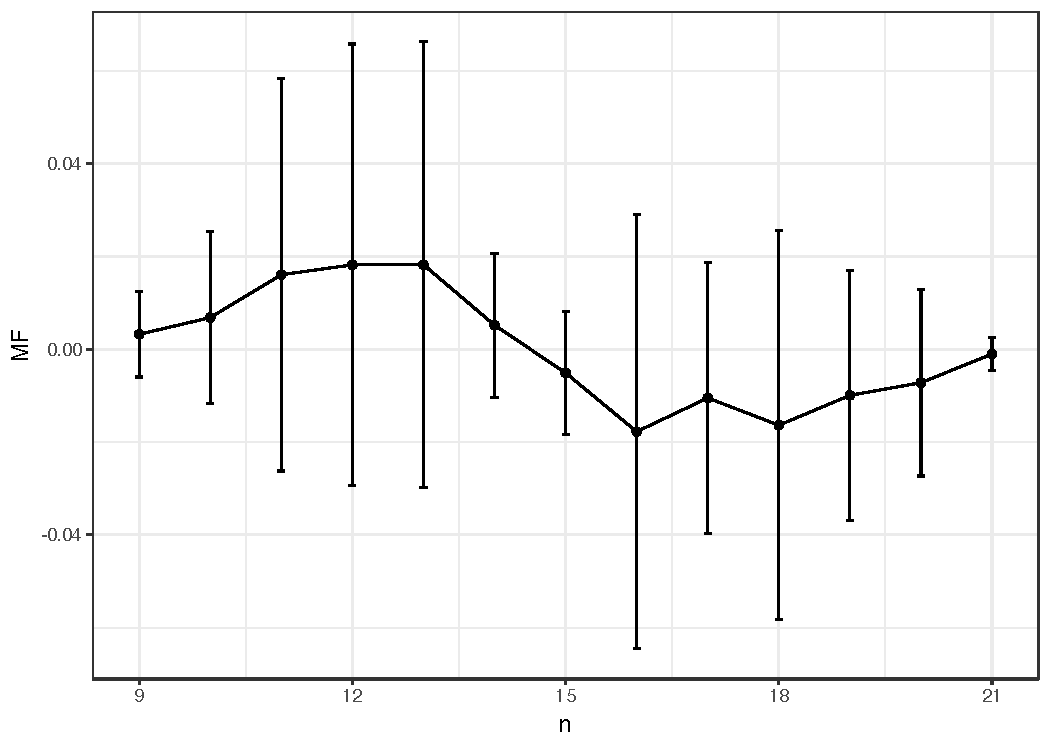
\includegraphics[width=0.5\textwidth]{mfx}
\label{f1}
\end{figure}

\item The second column of table \eqref{t6} shows  the ordered probit with only observed heterogeneity corresponding to profits of the form $\pi_{ik}(N)=X_{i}\beta+Z_{ik}\alpha+\delta ln(N)+v_{io}$. Notice that this  model fits the data better than the first model based on their log-likelihood measures. With this model we can see that the effect of the number of firms on profitability of entry is larger in magnitude. This means that profits decrease more if an additional firm enters compared to the first model. We also find presence at both endpoints of a route and share of miles traveled by a carrier increase the profitability of entry. As Berry mentions in his paper, this model uses the information of the equilibrium number of firm but can not distinguish the identities of entering firms. In fact ,it places a strong restriction on the difference in profits between entering and not entering firms:
\[
Z_{k}\alpha-Z_{j}\alpha>\delta(ln(N)-ln(N+1))
\]
This inequality suggests that if firm $k$ enters a market with an $N-$equilibrium and firm $j$ doesn't, then profits of firm $j$ can not be higher in  an $N+1$-equilibrium. Table \eqref{t7} shows that the rejection rate of the above inequality using the model with only observed heterogeneity is 55\%. This percentage is calculated using the following formula:
\[
\frac{\sum_{t=1}^{T}\sum_{k\in E_{t}}\sum_{j\in NE_{t}}\mathbf{1}\{Z_{k}\alpha-Z_{j}\alpha>\delta(ln(N)-ln(N+1))\}}{\sum_{t=1}^{T}|E_{t}||NE_{t}|}
\] 
where $E_{t}$ is the set of firms that enter market $t$, $NE_{t}$ is the set of firms that do not enter market $t$, and $|A|$ is the cardinality of set $A$. This relatively high rejection rate is an indication that the model with only observed heterogeneity is not suitable to explain the entry patterns in the data.

% Table generated by Excel2LaTeX from sheet 'Hoja1'
\begin{table}[H]
  \centering
  \caption{Restriction implied by the model with only observed heterogeneity}
    \begin{tabular}{lr}
    \hline
     Event     & Rejection rate \\
    \hline
    $\mathbf{1}\{Z_{k}\alpha-Z_{j}\alpha>\delta(ln(N)-ln(N+1))\}$ & 54,64\% \\
    \hline
    \end{tabular}%
  \label{t7}%
\end{table}

\item Table \eqref{t8} shows the estimation of the full model with simulations incorporating the order of entry moments as suggested in the appendix of Berry's paper. I do not estimate a moment condition between $v_{io}$ and the total city output share, hence I have 30 moment conditions unlike Berry who has 31.

% Table generated by Excel2LaTeX from sheet 'Hoja1'
\begin{table}[H]
  \centering
  \caption{Simulation estimates}
    \begin{tabular}{lr}
    \hline
          & Most profitable \\
          & move first\\
          \hline
    Constant & -1.0379 \\
    pop   & 1.4815 \\
    distance & 1.6017 \\
    city2 & 3.5467 \\
    sharepaxdist & 3.2772 \\
    $\delta$ & -2.2672 \\
    $\rho$   & 0.7003 \\
          \hline
    GMM Obj. Fun. & 5.0999 \\
    N     & 184 \\
    \hline
    \end{tabular}%
  \label{t8}%
\end{table}


\end{enumerate}


\end{document}